\documentclass[conference]{IEEEtran}
\IEEEoverridecommandlockouts
% The preceding line is only needed to identify funding in the first footnote. If that is unneeded, please comment it out.
\usepackage{cite}
\usepackage{amsmath,amssymb,amsfonts}
\usepackage{algorithmic}
\usepackage{graphicx}
\usepackage{textcomp}
\usepackage{xcolor}
\usepackage{tabularx}
\usepackage{multirow}
\usepackage{graphics} % for pdf, bitmapped graphics files
\usepackage{subfig}
\usepackage{subcaption}
\usepackage{hyperref}
\usepackage{academicons}
\usepackage{xcolor}
\usepackage{listings}
\def\BibTeX{{\rm B\kern-.05em{\sc i\kern-.025em b}\kern-.08em
		T\kern-.1667em\lower.7ex\hbox{E}\kern-.125emX}}
% Gráficas en MATLAB
\usepackage{tikz, pgfplots}
% Color Enlace
\definecolor{colorEnlace}{RGB}{0, 0, 0}
\hypersetup{
	colorlinks=true,
	linkcolor=colorEnlace,
	citecolor=colorEnlace,
	urlcolor=colorEnlace,
	pdfauthor={Ruth Juana Espino Puma},
	pdftitle={}
}
\lstset{
	language=Matlab, % Define el lenguaje
	basicstyle=\ttfamily\small, % Tamaño de letra pequeño
	keywordstyle=\color{blue}, % Color de las palabras clave
	commentstyle=\color{green}, % Color de los comentarios
	stringstyle=\color{red}, % Color de las cadenas de texto
	numbers=left, % Muestra los números de línea a la izquierda
	numberstyle=\tiny\color{gray}, % Estilo de los números de línea
	tabsize=1,
	stepnumber=1, % Muestra un número en cada línea
	breaklines=true, % Ajuste automático de línea
	frame=single, % Borde alrededor del código
	xleftmargin=0em, % Elimina el margen izquierdo
	framexleftmargin=0em % Elimina el espacio dentro del marco izquierdo
}
% Control 
\usepackage{amsmath}
\begin{document}
	
	\title{Experiencia N°6 - Controlador PD y PID}
	% Ing. Diego Darcy Arredondo Huarac
	\author{	
		\IEEEauthorblockN{Ruth Juana Espino Puma}
		\IEEEauthorblockA{Universidad Nacional de San Antonio Abad del Cusco}
		\textit{Escuela Profesional de Ingeniería Electrónica}\\
		\textit{Laboratorio de Control I}\\
		184657 \\\\
		Cusco, Perú
	}
	
	\maketitle
	
	\begin{abstract}
		The design of PD and PID controllers using root locus focuses on adjusting the closed-loop poles to achieve desired performance criteria such as stability, overshoot, settling time, and steady-state error. In PD controllers, the derivative action improves transient response by shifting poles to the left, increasing system damping. PID controllers, combining proportional, integral, and derivative actions, enhance both transient and steady-state performance. The root locus method aids in visualizing the impact of controller parameters on pole locations, allowing systematic tuning to meet design specifications.
	\end{abstract}
	
	\begin{IEEEkeywords}
		PD controller, PID controller, root locus, pole placement, transient response, steady-state error, damping ratio, system stability, tuning methods, control design
	\end{IEEEkeywords}
	
	\section{Introducción}
	
		Los controladores PD y PID son herramientas fundamentales en el control automático, ampliamente utilizados para mejorar el rendimiento de sistemas dinámicos. El controlador PD combina acciones proporcionales y derivativas, mejorando la respuesta transitoria al aumentar el amortiguamiento y acelerar el sistema sin afectar significativamente el error en estado estacionario. Por otro lado, el controlador PID agrega una acción integral que elimina el error en estado estacionario, logrando un equilibrio entre estabilidad, rapidez y precisión.
		
		El diseño de estos controladores mediante el lugar geométrico de las raíces (root locus) permite analizar gráficamente cómo se distribuyen los polos del sistema en función de los parámetros del controlador. Este enfoque facilita la ubicación estratégica de los polos en el plano complejo para cumplir con especificaciones de diseño como tiempo de asentamiento, sobrepaso máximo y estabilidad. El método no solo proporciona una comprensión visual del comportamiento del sistema, sino que también permite una sintonización más eficiente y precisa de los parámetros del controlador.
		
	\section{Objetivos}
	
	\begin{itemize}
		\item Diseñar Controlador PD y PID usando el Lugar Geométrico de las Raíces.
		\item Implementar Controlador PD y PID usando el Lugar Geométrico de las Raíces.
		\item Reducir el sobrepico a la mitad en función a los polos asignados mediante el diseño de un controlador PD y PID
	\end{itemize}
	
	\section{Usando el Lugar Geométrico de las Raíces diseñar Controlador PD y PID}
	
	El diseño de un compensador sin importa el método u origen, regla/norma que lo defina parte del deseo de modificar un sistema debido a que este no cumple con los requerimientos de funcionamiento definidos por lo cual es necesario modificar un parámetro del sistema (ganancia) para modificar su comportamiento o en segundo opción agregar un elemento adicional como un compensador cuando esto no es posible.
		
	Para el diseño del controlador PD y PID se hizo del lugar geométrico de las raíces el cual mediante la definición de los polos dominantes nos permiten modificar la respuesta del sistema para que se adecue a las necesidades de funcionamiento.
	
	\begin{itemize}
		\item Raices: $S_{1,2} = -10 \pm i15$
		\item $T_s = 0.4s$ (Tiempo de establecimiento)
		\item $M_p = 12.8\%$ (Sobreimpulso)
	\end{itemize}
	
	Siendo la función de transferencia del sistema a lazo abierto definida en \ref{eq:ft-planta} y mediante la cual podemos definir que se esta trabajando con un sistema de segundo orden, el cual tendrá un comportamiento inestable durante su estado transitorio, ello a causa al valor de su factor de amortiguamiento ubicado entre 0 y 1 y cual es equivalente a $\xi = 0.55$
	
	\begin{equation}
		H(s) = \frac{325}{s^2 + 20s + 325}
		\label{eq:ft-planta}
	\end{equation}
	
	Para la re-definición del sistema se tuvo en cuenta el comportamiento deseado siendo para el caso del sistema subamortiguado una reducción del sobreimpulso del este en un 50\% o la mitad del mismo, siendo así que al considerar este valor en conjunto con un $T_s = 0.22s$ tiempo de establecimiento arbitrario, se pudo calcular los polos dominantes o deseados mediante \ref{eq:polos-deseados}, además de que el calculo del nuevo factor de amortiguamiento $\xi = 0.66$ se calculo mediante \ref{eq:factor-amortiguamiento}.
	
	\begin{equation}
		S_{1,2} = -\xi \omega_n \pm j\omega \sqrt{1-\xi^2}
		\label{eq:polos-deseados}
	\end{equation}
	
	\begin{equation}
		\xi = \frac{-\ln(\frac{M_p}{100})}{\sqrt{\ln(\frac{M_p}{100})^2 + \pi^2}}
		\label{eq:factor-amortiguamiento} 	
	\end{equation}
	
	Para los polos dominantes en función a los 2 valores previamente calculados, se definieron:
	
	\begin{equation}
		s_{1,2} = -20 \pm j22.33 
		\label{eq:polos-dominates}
	\end{equation}
	
	Los polos dominantes serán de vital importancia para el diseño del controlador PD y PID debido a que nos permitirán realizar los cálculos matemáticos necesarios para establecer el lugar del cero en el caso el controlador PD y los ceros y el polo para el contexto del controlador PID.
	
	El diseño inicia con el análisis del lugar de las raíces para ver verificar si el sistema puede alterar su comportamiento o lo deseado mediante la variación de la ganancia del sistema u otro parámetro modificable, al analizar el LGR mostrado en la figura \ref{fig:lgr-planta} se puede apreciar que este no pasa por los polos deseados por lo que será necesario agregar un elemento adicional en cascada como lo es el controlador PD
	
	\begin{figure}[h]
		\centering
		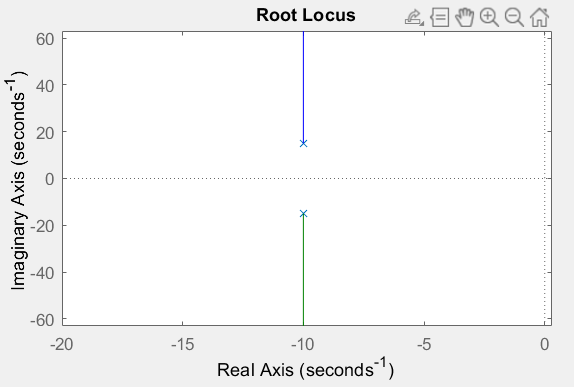
\includegraphics[width=0.5\textwidth]{media/lgr-planta.png}
		\caption{Lugar geométrico del sistema a lazo abierto}
		\label{fig:lgr-planta}
	\end{figure}
	
	Una vez definidos los polos y ceros en lazo abierto del sistema se definen los polos dominantes para calcular el angulo de compensación necesario para modificar el lugar geométrico del sistema de modo que este pase por los polos dominantes en lazo cerrado.
	
	Para el calculo del angulo de compensación se hace uso de la siguiente ecuación/sumatorias para ver en cuantos grados se tienen que compensar el sistema
	
	\begin{equation}
		\sum<Z -\sum<P = -180
		\label{eq:angulo-compensacion}
	\end{equation}
	
	Mediante \ref{eq:angulo-compensacion} se pudo determinar el angulo necesario para agregar mediante el controlador PD y/o PID y mediante ello determinar la ubicación de los cero faltante para cada caso, además para este calculo solo es necesario determinar el aporte en fase que aporte cada polo y zero, para el caso del controlador PD este aporte es de $\theta = 23.33º$ y para el caso del controlador PID este será $\theta = 86.474º$.
	
	Para calcular el resto de parámetros es necesario contar con la forma matemática del controlador PD y PID y las cuales se describen en \ref{eq:ft-pd} y \ref{eq:ft-pid}
	
	\begin{equation}
		G_r(s) = k(s + a)
		\label{eq:ft-pd}
	\end{equation}
	
	\begin{equation}
		G_s(s) = k_p + \frac{T_i}{s} + T_ds
		\label{eq:ft-pid}
	\end{equation}
	
	De ambas funciones de transferencia se puede destacar en concreto, estas cuenta con un factor de ganancia k o $k_p$ y las cuales se calcularan mediante la condición de magnitud definida en\ref{eq:condicion-magnitud} para cada caso, siendo así para que la primer caso se tiene un $k = 0.026706$ y para el segundo caso que incluye el integrador, se tiene un $k_p = 0.0049693$.
	
	\begin{equation}
		|G_r(s)G(s)| = 1
		\label{eq:condicion-magnitud}
	\end{equation}
	
	Sin embargo para poder calcular estas ganancias primero fue necesario determinar la ubicación exacta de los ceros y polos para caso, siendo así que se tienen las siguientes relaciones para cada caso.
	
	\subsection{Controlador PD}
	
	La ubicación del único cero una cantidad de unidades más allá del polo deseado, siendo a su vez que este se encuentra en función del angulo de compensación, al realizar la tangente del angulo de cero se puede calcular la ubicación del cero en el eje real negativo, mediante \ref{eq:cero-pd}
	\begin{align}
		x &= \frac{22.33}{tg(23.85)} \\ 
		x &= 50.5094 \\
		z &= 50.5094 + 20 \\
		z &= 70.5094 \\
		\label{eq:cero-pd}
	\end{align}
	Finalmente el controlador PD tendrá la siguiente forma siendo este el cual se colocara en cascada con el sistema para finalmente aplicar retroalimentación al sistema completo.
	
	\begin{equation}
		G_r(s) = 0.026706(s + 70.5094)
		\label{eq:ft-pd-1}
	\end{equation}
	\subsection{Controlador PID}
	Para el caso del controlador PID al estudiar la función de transferencia mediante \ref{ft-pid} se puede apreciar que por defecto se tiene un polo en el origen y 2 ceros (no necesariamente conjugados), en este punto se debe recordar es que el efecto de los ceros en un sistema de control es alejar el lugar del geométrico del semiplano derecho incrementando la estabilidad y reduciendo las oscilaciones en estado transitorio, por lo tanto para facilitar el calculo de uno de los ceros, hacemos uso del método de cancelación, el cual nos permitirá cancelar uno de los polos del sistema original, siendo necesario luego de ello solo el calculo de unos de los ceros mediante el método utilizado para el controlador PD y el cual se define en \ref{eq:cero-pid}
	\begin{align}
		x &= \frac{22.33}{tg(3.526)}\\
		x &= 362.3934 \\
		z &= 362.3934 + 20 \\
		z &= 382.3934
		\label{eq:cero-pid}
	\end{align}
	Siendo la función de transferencia del controlador PID la que se muestra en \ref{eq:ft-pd-1}
	\begin{equation}
		G_c(s) = \frac{0.0049693(s + 10)(s + 382.3934)}{s}
		\label{eq:ft-pid-1}
	\end{equation}
	
	Finalmente como es común con los sistemas de control mediante PD o PID será necesaria ua sintonización de sus constantes, por lo que para cada caso se modifico la ganancia para poder cumplir con los requisitos de funcionamiento para cada caso, para el caso del control PD se agrego un ganancia adicional de 20 y para el caso del PID una ganancia adicional de 0.66.
	
	\section{Simulación del sistema de control en lazo cerrado diseñado mediante MATLAB}
	Una forma de poder comprobar los resultados obtenidos y que los controladores calculados son los adecuados es mediante el uso de MATLAB, siendo así que el código para el controlador PD, se tiene:
	\begin{lstlisting}[numbers=none, caption={Controlador PD}]
		clear, clc;
		% Planta del sistema
		num = [325];
		den = [1 20 325];
		
		planta = tf(num, den)
		
		% Raices del sistema a lazo abierto
		raicesPlanta = roots(den);
		disp("Raices Planta:"+raicesPlanta);
		
		wnInicial = sqrt(num(1));
		xiInicial = den(2)/(2*wnInicial);
		tsInicial = 4/(wnInicial*xiInicial);
		fprintf("Parametros Iniciales\n\n");
		disp(["Freq. Natural Inicial: ", wnInicial]);
		disp(["Xi inicial: ", xiInicial]);
		disp(["Ts inicial: ", tsInicial]);
		
		fprintf("Nuevos parametros\n\n");
		% Parametros deseados
		mp = 6; % sobreimpulso
		ts = 0.20; % sobreimpulso
		errorTs =  abs(tsInicial-ts)*100/tsInicial; % El porcentaje de error entre los Ts (inicial y experimental)
		disp(["Error en el Ts: ", errorTs+"%"]);
		% Calculo de los nuevos parametros
		xi = -log(mp/100)/( sqrt(log(mp/100)^2 + pi^2) );
		wn = 4/(xi*ts);
		disp(["Xi: ", num2str(xi)]);
		disp(["Freq Natural: ", num2str(wn)]);
		
		% Calculo de los polos deseados
		pd = -xi*wn +i*wn*sqrt(1 - xi^2);
		disp(["Polo deseado: ", pd]);
		
		% Definiendo el Controlador PD
		zeroPD = [1 70.50];
		% Calculo de la ganancia
		ka = abs(evalfr(tf(den,zeroPD*num), pd));
		disp(["Ganancia PD: ", ka]);
		% Definiendo ganancia
		Gr = 20*ka*zeroPD
		
		sistema = tf( Gr*num , den)
		
		sistemaRetro = feedback(sistema,1)
		
		% Dibujando el LGR del sistema a lazo abierto
		figure(1); % Creando una figura
		subplot(2, 2, 1);
		rlocus(planta);
		subplot(2, 2, 2);
		rlocus(sistema);
		subplot(2, 2, 3);
		rlocus(sistemaRetro);
		
		% ================ =================== ================
		% ================ PROBANDO EL SISTEMA ================
		% ================ =================== ================
		figure(2); %
		tiempo_simulacion = 2;
		subplot(2, 1, 1);
		[resp_escalon_comp, t_escalon] = step(sistemaRetro, tiempo_simulacion);
		plot(t_escalon, resp_escalon_comp, 'b', 'DisplayName', 'Sistema Compensado');
		hold on;
		[resp_escalon_planta, t_escalon] = step(planta, tiempo_simulacion);
		plot(t_escalon, resp_escalon_planta, 'r', 'DisplayName', 'Planta');
		
		title('Respuesta al Escalon Unitario - Subamortiguado');
		xlabel('Tiempo (s)');
		ylabel('Amplitud');
		legend show;
		grid on; 
		hold off;
		
		% Subgrafica 2: Respuesta al impulso 
		subplot(2, 1, 2); 
		[resp_impulso_comp, t_escalon] = impulse(sistemaRetro, tiempo_simulacion);
		plot(t_escalon, resp_impulso_comp, 'b', 'DisplayName', 'Sistema Compensado');
		hold on;
		[resp_impulso_planta, t_escalon] = impulse(planta, tiempo_simulacion);
		plot(t_escalon, resp_impulso_planta, 'r', 'DisplayName', 'Planta');
		
		title('Respuesta al Impulso Unitario  - Subamortiguado');
		xlabel('Tiempo (s)');
		ylabel('Amplitud'); 
		legend show;
		grid on; 
		hold off;
		% Anadir titulo general 
		sgtitle('Respuestas Sistema subamortiguado con Retroalimentacion Unitaria');
	\end{lstlisting}
	
	Para el caso del controlador PID se tiene la siguiente simulación mediante MATLAB
	
	\begin{lstlisting}[numbers=none, caption={Controlador PID}]
		clear, clc;
		% Planta del sistema
		num = [325];
		den = [1 20 325];
		
		planta = tf(num, den)
		
		% Raices del sistema a lazo abierto
		raicesPlanta = roots(den);
		disp("Raices Planta:"+raicesPlanta);
		
		wnInicial = sqrt(num(1));
		xiInicial = den(2)/(2*wnInicial);
		tsInicial = 4/(wnInicial*xiInicial);
		fprintf("Parametros Iniciales\n\n");
		disp(["Freq. Natural Inicial: ", wnInicial]);
		disp(["Xi inicial: ", xiInicial]);
		disp(["Ts inicial: ", tsInicial]);
		
		fprintf("Nuevos parametros\n\n");
		% Parametros deseados
		mp = 6; % sobreimpulso
		ts = 0.20; % sobreimpulso
		errorTs =  abs(tsInicial-ts)*100/tsInicial; % El porcentaje de error entre los Ts (inicial y experimental)
		disp(["Error en el Ts: ", errorTs+"%"]);
		% Calculo de los nuevos parametros
		xi = -log(mp/100)/( sqrt(log(mp/100)^2 + pi^2) );
		wn = 4/(xi*ts);
		disp(["Xi: ", num2str(xi)]);
		disp(["Freq Natural: ", num2str(wn)]);
		
		% Calculo de los polos deseados
		pd = -xi*wn +i*wn*sqrt(1 - xi^2);
		disp(["Polo deseado: ", pd]);
		
		% Definiendo el Controlador PD
		zeroPID = [1 382.89];
		poloPID = [1 0];
		zeroPID1 = [1 10];
		
		gcZero = num*conv(zeroPID, zeroPID1);
		gcPolo = conv(poloPID, den);
		
		% Calculo de la ganancia
		ka = abs(evalfr(tf(gcPolo,gcZero), pd));
		disp(["Ganancia PD: ", ka]);
		
		% Definiendo ganancia
		
		sistema = tf(0.66*ka*gcZero, gcPolo )
		
		sistemaRetro = feedback(sistema,1)
		
		% Dibujando el LGR del sistema a lazo abierto
		figure(1); % Creando una figura
		subplot(2, 2, 1);
		rlocus(planta);
		subplot(2, 2, 2);
		rlocus(sistema);
		subplot(2, 2, 3);
		rlocus(sistemaRetro);
		
		% ================ =================== ================
		% ================ PROBANDO EL SISTEMA ================
		% ================ =================== ================
		figure(2); %
		tiempo_simulacion = 2;
		subplot(2, 1, 1);
		[resp_escalon_comp, t_escalon] = step(sistemaRetro, tiempo_simulacion);
		plot(t_escalon, resp_escalon_comp, 'b', 'DisplayName', 'Sistema Compensado');
		hold on;
		[resp_escalon_planta, t_escalon] = step(planta, tiempo_simulacion);
		plot(t_escalon, resp_escalon_planta, 'r', 'DisplayName', 'Planta');
		
		title('Respuesta al Escalon Unitario - Subamortiguado');
		xlabel('Tiempo (s)');
		ylabel('Amplitud');
		legend show;
		grid on; 
		hold off;
		
		% ============= =========== =========
		% Subgrafica 2: Respuesta al impulso
		% ============= =========== =========
		subplot(2, 1, 2); 
		[resp_impulso_comp, t_escalon] = impulse(sistemaRetro, tiempo_simulacion);
		plot(t_escalon, resp_impulso_comp, 'b', 'DisplayName', 'Sistema Compensado');
		hold on;
		[resp_impulso_planta, t_escalon] = impulse(planta, tiempo_simulacion);
		plot(t_escalon, resp_impulso_planta, 'r', 'DisplayName', 'Planta');
		
		title('Respuesta al Impulso Unitario  - Subamortiguado');
		xlabel('Tiempo (s)');
		ylabel('Amplitud'); 
		legend show;
		grid on; 
		hold off;
		% Anadir titulo general 
		sgtitle('Respuestas Sistema subamortiguado con Retroalimentacion Unitaria');
		
	\end{lstlisting}
	
	En cada caso de forma general se muestran el lugar geométrico del sistema original, del sistema retroalimentado luego de aplicar en cascada el controlador PID y finalmente la respuesta del sistema frente al impulso unitario y el escalón unitario.
	
	\section{Mostrar las gráficas del ítem anterior, ¿Cuál es la explicación de estas graficas?}
	Como se puede apreciar en la figura \ref{fig:respuesta-sistema} se puede apreciar la respuesta del sistema frente a una excitación de entrada del tipo escalón e impulso unitario, 
	
	\begin{figure}[h]
		\centering
		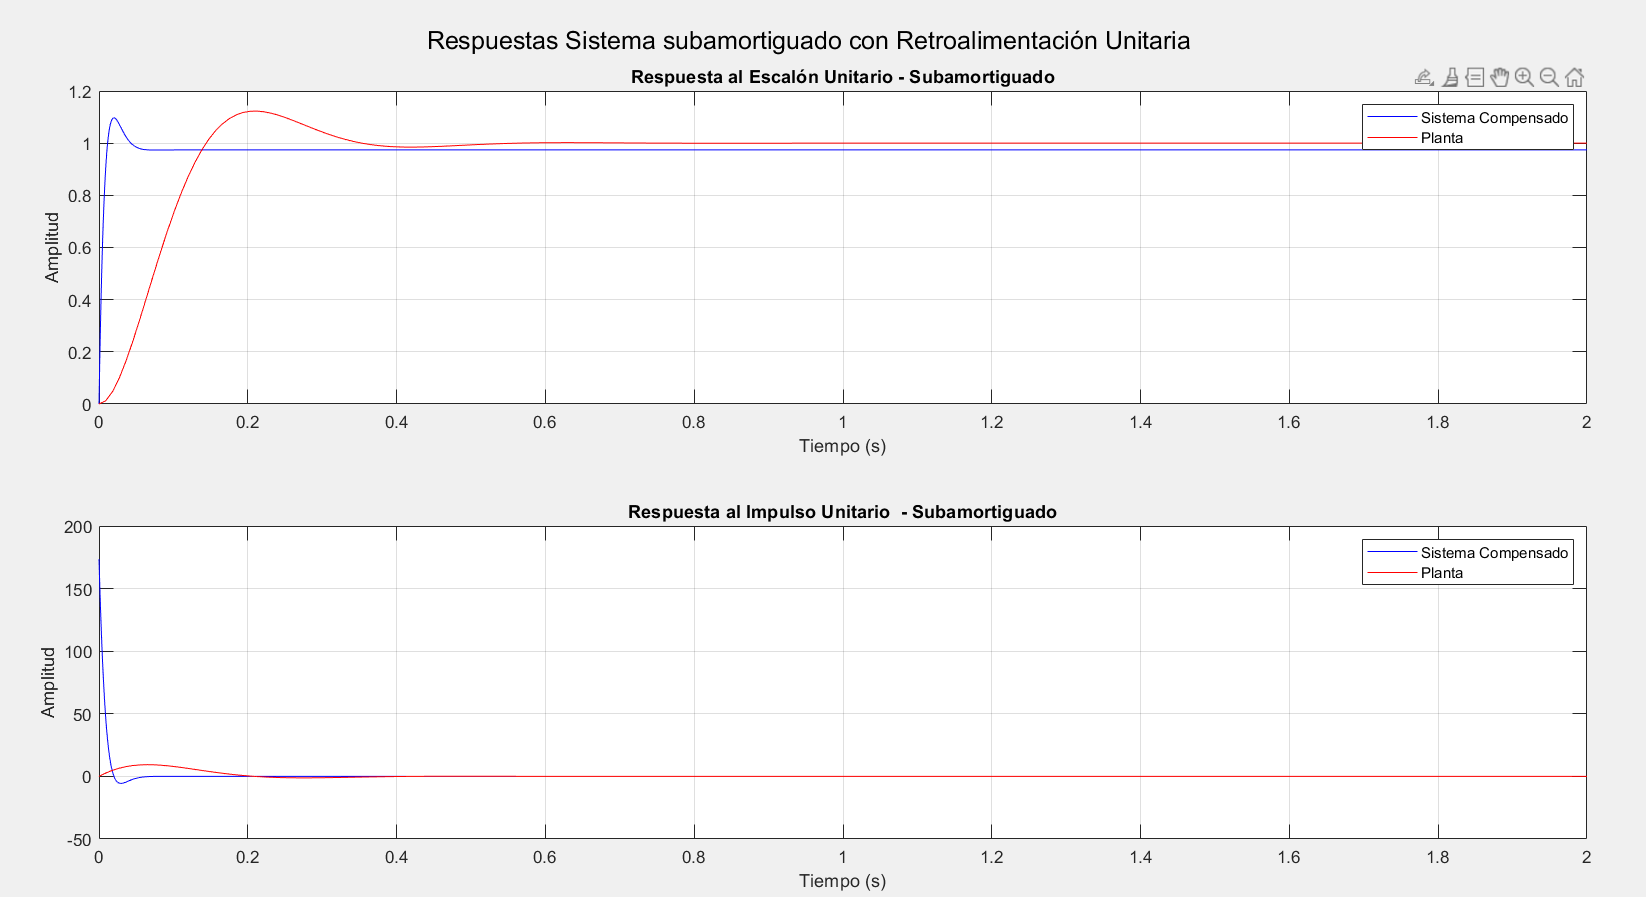
\includegraphics[width=0.5\textwidth]{media/respuesta-sistema.png}
		\caption{Respuesta del sistema al escalón e impulso unitario}
		\label{fig:respuesta-sistema}
	\end{figure}
	De la gráfica se puede apreciar que sistema original presenta un comportamiento subamortiguado típico, con oscilaciones iniciales notorias y un sobrepaso antes de estabilizarse y por otro lado el sistema original presenta un comportamiento subamortiguado típico, con oscilaciones iniciales notorias y un sobrepaso antes de estabilizarse y en la cual se puede apreciar una reducción el sobreimpulso y una aceleración en el tiempo de establecimiento.
	
	\bibliographystyle{IEEEtran}
	\bibliography{biblio}
\end{document}



































